El circuito electrónico construido para el sistema está resumido en la \autoref{fig:hardware/montaje/bloquesSimples}. En ella se puede ver que se tiene la entrada solar, la cual puede cargar la batería de \textit{Backup} y un seleccionador de entrada para el sistema, que puede alimentarse de la tensión solar o de la batería de \textit{Backup}. De esta entrada se alimentan los dos cargadores de las baterías y el microcontrolador. Además, el módulo del microcontrolador alimenta los sensores de tensión y corriente, se comunica con el bus \texttt{I2C} e interactúa con los relés.

\begin{figure}[H]
    \centering
    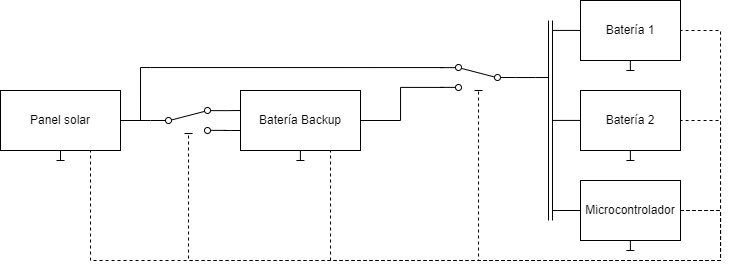
\includegraphics[width=0.95\textwidth]{images/2-hardware/bloquesSimples.png}
    \caption{Diagrama de bloques simples del sistema}
    \label{fig:hardware/montaje/bloquesSimples}
\end{figure}